Man kann als Anfang des Onlinehandels 3 Daten ansetzen. Um 1970 haben Standfort Studenten mit Studenten der Universität Massachusetts ein Geschäft auf den Internet Vorgänger Arpanet abgewickelt. Das erworbene Produkt war ein Tütchen Marihuana. Ein weiteren Zwischenschritt zur kompletten offiziellen Einführung eines online Marktplatzes war ein Pilotenprogramm, worin Jane Snowballs Fernseher mit einem System gekoppelt worden ist wodurch es der 72-jährige möglich gemacht wurde durch den Teletext bei dem lokalen Lebensmittelunternehmen Tesco Lebensmittel zu bestellen. Ihre erste Bestellung war Margarine, Eier und Cornflakes. Die erste offizielle Onlinemarkttransaktion wurde auf Netmarket beim Händler Noteworty Musics abgewickelt. Beim dem zu verkaufenden Produkt handelte es sich um eine CD der Band Sting namens "Ten Summoner´s Tales" \cite{bihler}. Durch diese Grundstrukturen hat sich ein Wirtschaftssektor gebildet der profitabelste Sektor für ein großes Unternehmen ist. Besonders durch die Einbeziehung des Onlinehandels konnte der E-Commerce erst seinen Aufstieg feiern. Jedoch ist das Potential des Sektors noch lange nicht ausgeschöpft. Durch die Entwicklung von Sprachassistenten und Künstlichen Intelligenzen wird die Zeit des Prozesses des Einkaufens bis zum minimalen verringert. Auch durch das Integrieren von Drohen wird die Allgegenwärtigkeit des Onlinehandels früher oder später offensichtlich \cite{leopold}. Die Steigerung des Kommerzes, ins besonderen in ländlichen Regionen ist überwältigend. Vom Jahr 2000 bis 2020 hat sich der Umsatz in Deutschland mehr als verfünfzigfacht. Von 1,3 Milliarden € auf 59,2 Milliarden € in nur zwanzig Jahren \cite{poleshov}. Auch zeigen die Tendenzen der Nutzer in den kommenden Jahren nur nach oben. Bis 2023 sollen 71,4 Millionen Deutsche online einkaufen.

 \begin{figure}[h]
    \begin{center}
        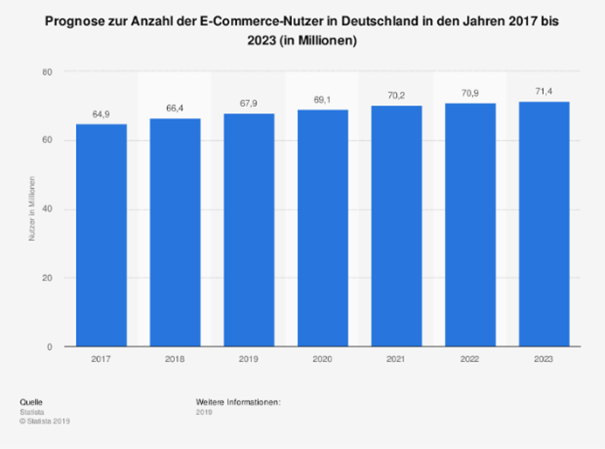
\includegraphics[width=8cm]{media/1.png}
        \caption{Prognose der Nutzer des E-Commerce}
        \label{Prognose Nutzer}
        \bildquelle  Prognose zur Anzahl der E-Commerce Nutzer in Deutschland in den Jahren 2017 bis 2023 (in Millionen) In: Parcellab (2019). https://bit.ly/2MgpATh - aufgerufen am 28. 12. 2020
    \end{center}
\end{figure}



\noindent Jedoch hat der Onlinehandel auch durch Modernisierung und Entwicklung als auch die Verbreitung unserer Smartphones und anderen elektrischen Geräte so einen großen Umsatz erzielt. Auch In-App-Käufe tragen einen Teil bei. Ebenfalls ist es auch ein Markt dessen Potential noch nicht ausgeschöpft ist. Von 2016 zu 2018 haben die In-App-Käufe weltweit einen Zuwachs von 75\% erreicht was eine Steigerung von knapp 70 Milliarden \$ heißt.

 \begin{figure}[h]
    \begin{center}
        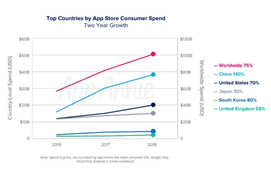
\includegraphics[width=8cm]{media/2.png}
        \caption{Länder beim App-Store-Kauf}
        \label{Länder Ranking}
        \bildquelle Top Countries by App Store Consumer Spend In: Onlinemarketing.de (2019). https://bit.ly/38F6qhm - aufgerufen am 28. 12. 2020
    \end{center}
\end{figure}


\noindent Speziell in Ländern wie China oder den USA haben sich In-App-Käufe verbreitet. Besonders Spotify Sticht unter den Apps heraus mit einem Wert von 29,5 Milliarden. 

 \begin{figure}[h]
    \begin{center}
        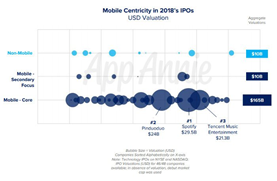
\includegraphics[width=8cm]{media/3.png}
        \caption{Meist gekauften App-Dienste }
        \label{App-Dienste}
        \bildquelle Mobile Centricity in 2018´s IPOs. https://bit.ly/34QkIuw - aufgerufen am 28. 12. 2020
    \end{center}
\end{figure}

Hingegen sind Video-Streaming-Dienste momentan im Trend da sie ihren Nutzern, durch Werbung, Echtgeld bezahlen können, dass sie bereits durch das Schalten der Werbung bei den Videos verdient haben.

\begin{figure}[h]
    \begin{center} 
        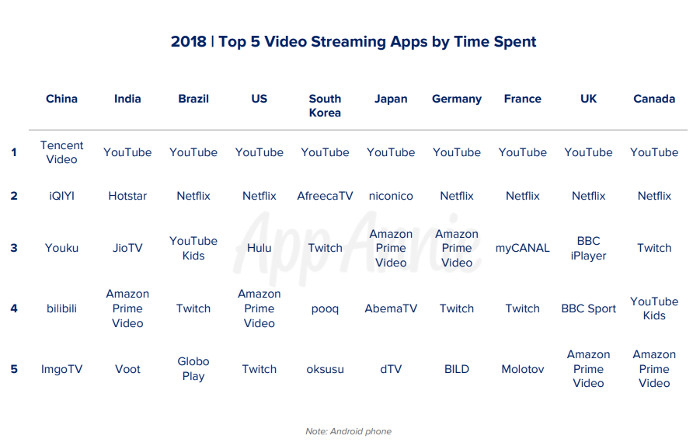
\includegraphics[width=10cm]{media/4.png}
        \caption{Top 5 Video Streaming Apps by Time Spent}
        \label{stream}
        \bildquelle Extremes Wachstum im Mobile Marketing: Nutzungszeit und Ausgaben steigen rasant. In: Onlinemarkting.de (2019). https://bit.ly/2KxUiH9. – aufgerufen am 25. 12. 2020
    \end{center}
\end{figure}
  
\noindent In Deutschland ist Youtube bereits seit Jahren der Spitzenreiter, wenn es um Video-Streaming geht. Weltweit macht das Unternehmen 6 Milliarden \$ Umsatz im Jahr 2015.
